%!mode::"TeX:UTF-8"
\documentclass[a4paper]{article}
\usepackage[fntef]{ctexcap} % Required for the Chinese and the corresponding section setting
\usepackage[top=2.5cm, bottom=2.5cm, left=2.5cm, right=2.5cm]{geometry} % Required for the Word-like page
\usepackage{fancyhdr} % Required for custom headers
\usepackage{setspace} % Required for the space setting
\usepackage{titlesec} % Required for the Chapter & Section fonts adjustment
\usepackage{titletoc} % Required for the Content fonts adjustment
\usepackage[toc,page]{appendix} % Required for the appendix environment
\usepackage{lastpage} % Required to determine the last page for the footer
\usepackage{extramarks} % Required for headers and footers
\usepackage{courier} % Required for the courier font
\usepackage{float} % Required for the Here float
\usepackage{graphicx} % Required to insert images
\usepackage{wrapfig}
\usepackage{booktabs} % Required for the hline of the three lines table
\usepackage{multirow} % Required for the multirow of table
\usepackage{listings} % Required for insertion of code
\usepackage{indentfirst} % Required for the indent before each paragraph
\usepackage[bookmarks=true,colorlinks=true,linkcolor=black,anchorcolor=blue,citecolor=blue,urlcolor=blue]{hyperref}
%\usepackage{cite} % Required for the ref and cite
\usepackage[usenames,dvipsnames]{color} % Required for custom colors
\usepackage{courier} % Required for the courier font
\usepackage[font=footnotesize,tableposition=top]{caption} % Required for the footnote size captions of figures and tables
\usepackage[numbers,sort&compress]{natbib}
%----------------------------------------------------------------------------------------
%   Math Display
%----------------------------------------------------------------------------------------
\usepackage{bm} % Required for the bold in math display
\usepackage{amsmath} % Required for the math display
\usepackage{amssymb} % Required for the math display
\usepackage{amsbsy} % Required for the math display
\usepackage{cancel} % Required for the cancel symbol in math display
\usepackage{amsthm} % Required for the theorem edition
\usepackage{array} % Required for the array in math display
\usepackage{ifthen} % Required for the conditional commands


%----------------------------------------------------------------------------------------
%   Superscript citation
%----------------------------------------------------------------------------------------
\newcommand{\upcite}[1]{\textsuperscript{\textsuperscript{\cite{#1}}}}

%----------------------------------------------------------------------------------------
%   Upright d in integrate
%----------------------------------------------------------------------------------------
\newcommand{\ud}{\mathrm{d}} 

%----------------------------------------------------------------------------------------
%   Code Inclusion Configuration
%----------------------------------------------------------------------------------------
\definecolor{MyDarkGreen}{rgb}{0.0,0.4,0.0} % This is the color used for comments
\lstloadlanguages{Python} % Load Python syntax for listings, for a list of other languages supported see: ftp://ftp.tex.ac.uk/tex-archive/macros/latex/contrib/listings/listings.pdf
\lstset{language=Python, % Use Python in this example
frame=single, % Single frame around code
%basicstyle=\ttfamily, % Use small true type font
keywordstyle=[1]\color{Blue}\bf, % Python functions bold and blue
keywordstyle=[2]\color{Purple}\it, % Python function arguments purple
keywordstyle=[3]\color{Blue}\underbar, % Custom functions underlined and blue
identifierstyle=, % Nothing special about identifiers                                         
commentstyle=\color{Gray}, % Comments small dark green courier font
stringstyle=\color{Green}, % Strings are purple
showstringspaces=false, % Don't put marks in string spaces
tabsize=4, % 4 spaces per tab
% Put standard Python functions not included in the default language here
morekeywords={rand},
% Put Python function parameters here
morekeywords=[2]{on, off, interp},
% Put user defined functions here
morekeywords=[3]{test},
%
morecomment=[l][\color{Blue}]{...}, % Line continuation (...) like blue comment
numbers=left, % Line numbers on left
firstnumber=1, % Line numbers start with line 1
numberstyle=\tiny\color{Blue}, % Line numbers are blue and small
stepnumber=1 % Line numbers go in steps of 1
}
% Creates a new command to include a Python script, the first parameter is the filename of the script (without .py), the second parameter is the caption
\newcommand{\pythonscript}[2]{
\begin{itemize}
\begin{spacing}{1.0}
\item[]\lstinputlisting[caption=#2,label=#1]{#1.py}
\end{spacing}
\end{itemize}
}

%----------------------------------------------------------------------------------------
%   Section related equations' number
%----------------------------------------------------------------------------------------
\makeatletter
\@addtoreset{equation}{section}
\makeatother
\renewcommand{\theequation}{\arabic{section}.\arabic{equation}}

%----------------------------------------------------------------------------------------
%   Chapter & Section fonts adjustment
%----------------------------------------------------------------------------------------
\CTEXsetup[name={第,章},number={\chinese{section}},format={\centering\zihao{-2}\bfseries}]{section}
\titleformat{\subsection}{\zihao{-3}\bfseries}{\thesubsection}{1em}{}
\titleformat{\subsubsection}{\zihao{4}\bfseries}{\thesubsubsection}{1em}{}
\CTEXsetup[,format={\raggedright\bfseries\zihao{-4}}]{paragraph}
%----------------------------------------------------------------------------------------
%   Content fonts adjustment
%----------------------------------------------------------------------------------------
\renewcommand\contentsname{目\quad\quad 录} % Setup contents
\titlecontents{section}[0em]{\zihao{4}\bfseries}{\contentspush{\thecontentslabel \hspace{0.7em}}}
              {}{\titlerule*[5pt]{.}\contentspage}
\titlecontents{subsection}[2.2em]{\zihao{-4}\songti}{\contentspush{\thecontentslabel\hspace{0.7em}}}
              {}{\titlerule*[5pt]{.}\contentspage}
\titlecontents{subsubsection}[3.9em]{\zihao{-4}\songti}{\contentspush{\thecontentslabel\hspace{0.7em}}}
              {}{\titlerule*[5pt]{.}\contentspage}
\titlespacing*{\subsection} {0pt}{1ex}{1ex} % Adjust the space between title and context
\titlespacing*{\subsubsection} {0pt}{1ex}{1ex}

%----------------------------------------------------------------------------------------
%   Page header & Page footer setting
%----------------------------------------------------------------------------------------
\pagestyle{fancy}
\fancyhf{}
\renewcommand{\sectionmark}[1]{\markboth{第\chinese{section} 章{\color{white}.} #1}{}}
\fancyhead[C]{\CJKfamily{song}华南理工大学学士学位论文}
\fancyhead[CO]{\CJKfamily{song}\leftmark}
\fancyfoot[C]{\thepage}

\begin{document}
%----------------------------------------------------------------------------------------
%   Cover
%----------------------------------------------------------------------------------------
\thispagestyle{empty}
\begin{figure}[ht]
\centering

\includegraphics[height=2.75cm]{title.png}
\end{figure}
\begin{center}
\zihao{0}
\textbf{本科毕业论文}
\end{center}
\nopagebreak[4]
\begin{center}
\zihao{1}
\ \\
\end{center}
\nopagebreak[4]
\begin{center}
\zihao{2}
\textbf{你的本科毕业论文题目}
\end{center}
\nopagebreak[4]
\begin{center}
\zihao{1}
\ \\\ \\\ \\
\end{center}
\nopagebreak[4]
\begin{spacing}{1.8}
\begin{center}
\zihao{-3}
% Via \quad, \qquad or '\ ' (backslash and space) you can adjust the length of the line
\textbf{学\quad\quad 院}\quad\underline{\quad\quad\textbf{你的学院}\quad\quad}\\
\textbf{专\quad\quad 业}\quad\underline{\quad\quad\quad\textbf{你的专业全称}\quad\quad\quad}\\
\textbf{学生姓名}\quad\underline{\quad\quad\quad\quad\textbf{你的名字}\quad\quad\quad\quad}\\
\textbf{学生学号}\quad\underline{\quad\quad\textbf{201abcdefghi}\quad\quad}\\
\textbf{指导老师}\quad\underline{\quad\quad\textbf{导师1,\ 导师2}\quad\quad}\\
\textbf{提交日期}\quad\underline{\quad\textbf{2000年}\ \ \textbf{00月}\ \ \textbf{00日}\quad}
\end{center}
\end{spacing}
\pagebreak[4]

%----------------------------------------------------------------------------------------
%   Chinese Abstract
%----------------------------------------------------------------------------------------
\setcounter{page}{1}
\pagenumbering{Roman}
\begin{center}
\addcontentsline{toc}{section}{摘要} % Add to content
\zihao{-2}
\bfseries
 摘\quad 要
\end{center}
\thispagestyle{plain}
\begin{spacing}{1.5}
\zihao{-4}
摘要内容应概括地反映出本论文的主要内容, 主要说明本论文的研究目的、内容、方法、成果和结论. 要突出本论文的创造性成果或新见解, 不要与引言相混淆. 语言力求精练、准确,以300-500字为宜. 在摘要的下方另起一行, 注明本文的关键词 (3-5个). 关键词是供检索用的主题词条, 应采用能覆盖论文主要内容的通用技术词条 (参照相应的技术术语标准). 按词条的外延层次排列 (外延大的排在前面). 摘要与关键词应在同一页.
\ \\
\textbf{关键词: }多变量系统; 预测控制; 环境试验设备
\end{spacing}
\pagebreak[4]
\thispagestyle{plain}

%----------------------------------------------------------------------------------------
%   English Abstract
%----------------------------------------------------------------------------------------
\begin{center}
\addcontentsline{toc}{section}{Abstract} % Add to content
\zihao{-2}
Abstract
\end{center}
\begin{spacing}{1.5}
\zihao{-4}
英文摘要内容与中文摘要相同, 以 250-400个实词为宜. 摘要下方另起一行注明英文关键词 (Keywords3-5个).
\ \\
\textbf{Keywords: }Writer recognition; Convolutional Neural Network; Handwritten character recognition
\end{spacing}
\pagebreak[4]

%----------------------------------------------------------------------------------------
%   CONTENTS
%----------------------------------------------------------------------------------------
\thispagestyle{plain}
\begin{spacing}{1.5}
\addcontentsline{toc}{section}{目录}
\tableofcontents
\end{spacing}
\thispagestyle{plain}
\pagebreak[4]

%----------------------------------------------------------------------------------------
%   BEGIN TO COUNT THE PAGE NUMBER
%----------------------------------------------------------------------------------------
\setboolean{@twoside}{true}
\begin{spacing}{1.5}
\zihao{-4}
\setcounter{page}{1}
\pagenumbering{arabic}
%----------------------------------------------------------------------------------------
%   BELOW IS YOUR MAIN TEXT. BEGIN.
%----------------------------------------------------------------------------------------

%----------------------------------------------------------------------------------------
%   绪论
%----------------------------------------------------------------------------------------
\section{绪论}
%----------------------------------------------------------------------------------------
%   选题背景与意义
%----------------------------------------------------------------------------------------
\subsection{选题背景与意义}
\label{sec:background}
引言是论文正文的开端, 应包括毕业论文选题的背景、目的和意义; 对国内外研究现状和相关领域中已有的研究成果的简要评述; 介绍本项研究工作研究设想、研究方法或实验设计、理论依据或实验基础; 涉及范围和预期结果等. 要求言简意赅,注意不要与摘要雷同或成为摘要的注解.

%----------------------------------------------------------------------------------------
%   国内外研究现状和相关工作
%----------------------------------------------------------------------------------------
\subsection{国内外研究现状和相关工作}
\label{sec:related_work}
对国内外研究现状和相关领域中已有的研究成果的简要评述

%----------------------------------------------------------------------------------------
%   本文的论文结构与章节安排
%----------------------------------------------------------------------------------------
\subsection{本文的论文结构与章节安排}
\label{sec:arrangement}
本文共分为五章, 各章节内容安排如下:

第一章引言.

第二章知识点.

第三章方法介绍.

第四章实验和结果.

第五章是本文的最后一章, 总结与展望. 是对本文内容的整体性总结以及对未来工作的展望.

\pagebreak[4]


\section{数据}

%----------------------------------------------------------------------------------------
%   本文的论文结构与章节安排
%----------------------------------------------------------------------------------------
\section{简单的使用例子}
\label{cha:example}
%----------------------------------------------------------------------------------------
%   图像的插入
%----------------------------------------------------------------------------------------
\subsection{图像的插入}
\label{sec:Images}
\begin{wrapfigure}{r}{0.5\linewidth}
\centering
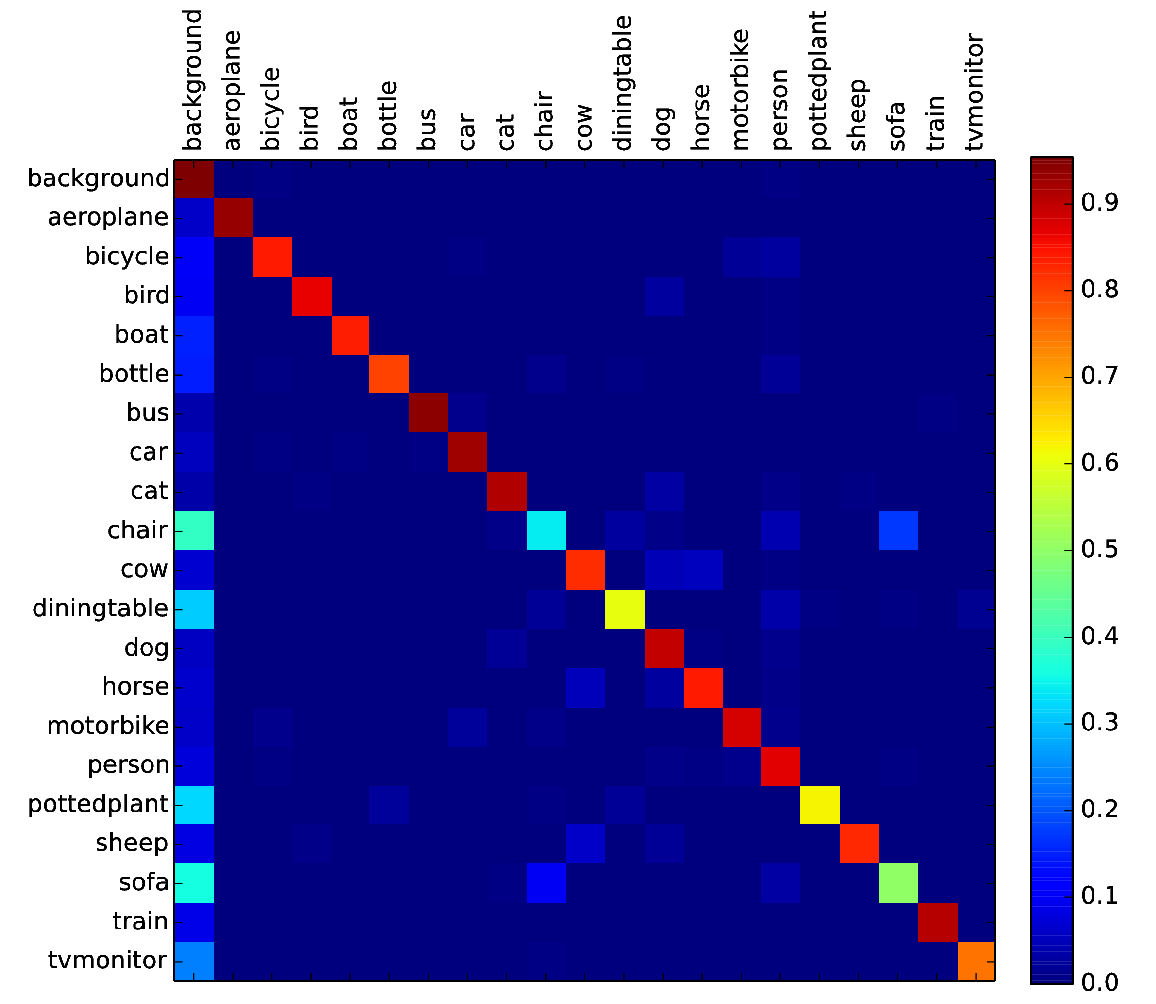
\includegraphics[width=0.5\textwidth]{images/Chap2/confusion.pdf} % width=0.5\textwidth也可以换成width=5cm, height=5cm等关键字参数. width=0.5\textwidth 比较常用: 图片宽度等于你的text宽度的1/2
\caption{镶嵌在文中的图像}
\label{fig:confusion}
\end{wrapfigure}
论文主体是毕业论文的主要部分, 必须言之成理, 论据可靠, 严格遵循本学科国际通行的学术规范. 在写作上要注意结构合理、层次分明、重点突出, 章节标题、公式图表符号必须规范统一. 论文主体的内容根据不同学科有不同的特点, 一般应包括以下几个方面: (1)毕业论文 (设计) 总体方案或选题的论证; (2)毕业论文 (设计) 各部分的设计实现, 包括实验数据的获取、数据可行性及有效性的处理与分析、各部分的设计计算等; (3)对研究内容及成果的客观阐述, 包括理论依据、创新见解、创造性成果及其改进与实际应用价值等; (4)论文主体的所有数据必须真实可靠, 凡引用他人观点、方案、资料、数据等, 无论曾否发表, 无论是纸质或电子版, 均应详加注释. 自然科学论文应推理正确、结论清晰; 人文和社会学科的论文应把握论点正确、论证充分、论据可靠, 恰当运用系统分析和比较研究的方法进行模型或方案设计, 注重实证研究和案例分析, 根据分析结果提出建议和改进措施等.

可以插入单张图像:
\begin{figure}[h]
\centering
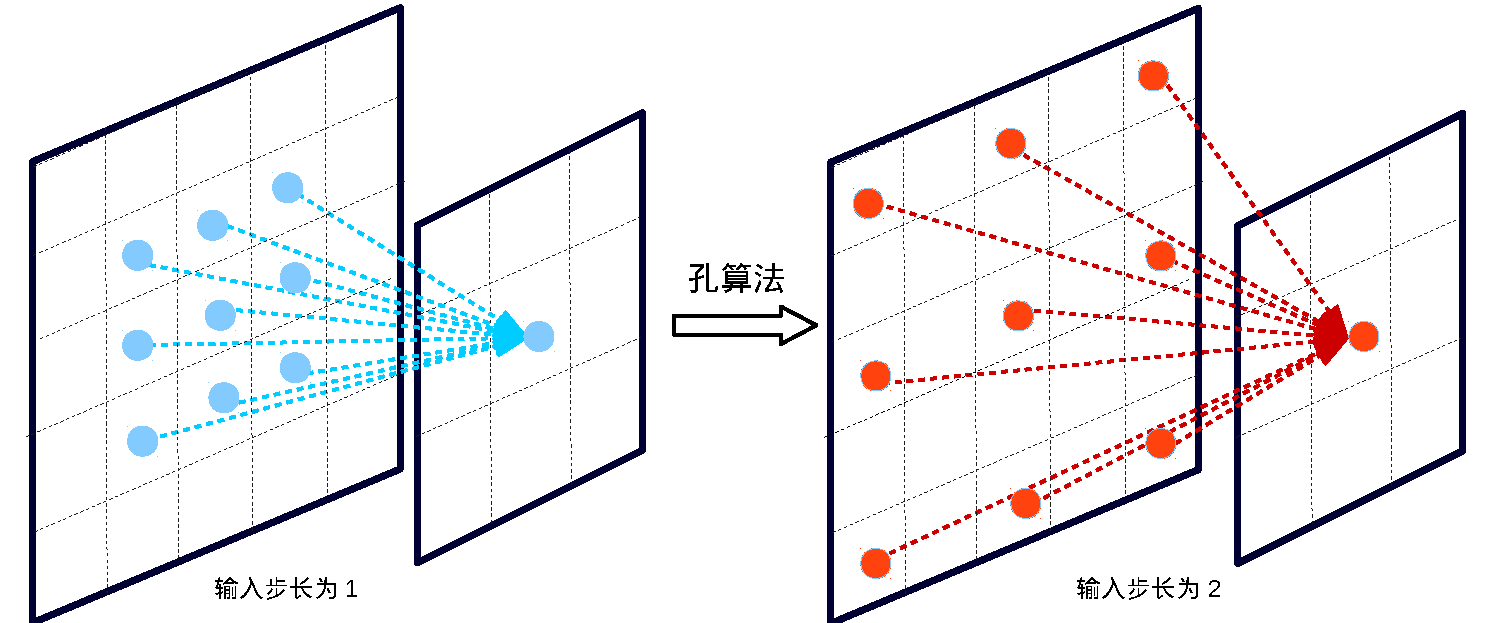
\includegraphics[width=0.5\textwidth]{images/Chap2/hole.pdf}
\caption{单张图像}
\label{fig:hole}
\end{figure}



\pagebreak[4]%换页
\appendix
\section{Markov Chain}
一个理论值$X^H(\vec{\theta})$是参数列$\vec{\theta}$的函数, $\vec{\theta}$是$M$维空间的矢量:
\begin{equation}
\vec{\theta}=[\theta_1, \theta_2, ..., \theta_M]
\end{equation}


\pagebreak[4]%换页

%----------------------------------------------------------------------------------------
%   CERN
%----------------------------------------------------------------------------------------

\section{CERN}
了.


%正文内容到此为止
\end{spacing}
\setboolean{@twoside}{false}
%正文结束
\fancyhead[C]{\CJKfamily{song}华南理工大学学士学位论文}
\fancyhead[CO]{\CJKfamily{song}\leftmark}


%插入参考文献
\pagebreak[4]
\begin{thebibliography}{99}
\addcontentsline{toc}{section}{参考文献}
\zihao{-4}
%\tnewroman

%----------------------------------------------------------------------------------------
%   绪论
%----------------------------------------------------------------------------------------

\bibitem{Oh-My-God Particles} \href{https://www.universetoday.com/86490/astronomy-without-a-telescope-oh-my-god-particles/}{Astronomy Without A Telescope - Oh-My-God Particles - Universe Today}


\end{thebibliography}


\pagebreak[4]
%=====================致谢=============================%
\thispagestyle{empty}
\section*{致谢}
\addcontentsline{toc}{section}{致谢}%将“摘要加入目录中”
\begin{spacing}{1.5}
\zihao{-4}
\songti
Time flies very fast, 很惭愧, 其实我只做了一点微小的工作.
\end{spacing}
\end{document}
